%
% collection of useful formulas
% @author Tobias Weber <tweber@ill.fr>
% @date 13-jul-2018
% @license see 'LICENSE' file
%

\documentclass{article}

\usepackage{amsmath}
\usepackage{graphicx}

\usepackage[a4paper]{geometry}
\geometry{tmargin=2.5cm, bmargin=2.5cm, lmargin=2cm, rmargin=2cm}


\begin{document}
Collection of useful formulas, T. Weber, July 13, 2018.


\section{Scattering Triangle}
\begin{center}
	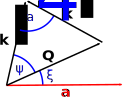
\includegraphics[width = 0.2 \textwidth]{triangle}
\end{center}


\subsection*{Scattering Angle $a_4$}

\begin{equation} \left| Q \right> = \left| k_i \right> - \left| k_f \right> \\ \end{equation}
\begin{equation} \left< Q | Q \right> = \left( \left< k_i \right| - \left< k_f \right| \right) \cdot \left( \left| k_i \right> - \left| k_f \right> \right) \end{equation}
\begin{equation} \left< Q | Q \right> = \left< k_i | k_i \right> + \left< k_f | k_f \right> - 2 \left< k_i | k_f \right> \end{equation}
\begin{equation} Q^2 = k_i^2 + k_f^2 - 2 k_i k_f \cos a_4 \end{equation}
\begin{equation} \boxed{ a_4 = \arccos \left( \frac{k_i^2 + k_f^2 - Q^2}{2 k_i k_f} \right) } \end{equation}



\subsection*{Rocking Angle $a_3$}

\begin{equation} \boxed{ a_3 = 180^{\circ} - \left( \psi + \xi \right) } \end{equation}

Angle $\psi$ between $\left| k_i \right>$ and $\left| Q \right>$, in units of \AA{}$^{-1}$, as before:
\begin{equation} \left| k_f \right> = \left| k_i \right> - \left| Q \right> \end{equation}
\begin{equation} \left< k_f | k_f \right> = \left( \left< k_i \right| - \left< Q \right| \right) \cdot \left( \left| k_i \right> - \left| Q \right> \right) \end{equation}
\begin{equation} \left< k_f | k_f \right> = \left< k_i | k_i \right> + \left< Q | Q \right> - 2 \left< k_i | Q \right> \end{equation}
\begin{equation} k_f^2 = k_i^2 + Q^2 - 2 k_i Q \cos \psi \end{equation}
\begin{equation} \boxed{ \psi = \arccos \left( \frac{k_i^2 + Q^2 - k_f^2}{2 k_i Q} \right) } \end{equation}

Angle $\xi$ between $\left| Q \right>$ and orientation vector $\left| a \right>$ (i.e. $ax$, $ay$, $az$), in units of rlu; $g_{ij} = \left| b_i \left> \right< b_j \right|$ is the covariant metric of the reciprocal lattice with basis $\left| b_i \right>$:
\begin{equation} \xi = \arccos \left( \frac{ \left< Q | a \right> }{ \sqrt{\left< Q | Q \right>} \sqrt{\left< a | a \right>} } \right) \end{equation}
\begin{equation} \boxed{ \xi = \arccos \left( \frac{ Q^i g_{ij} a^j }{ \sqrt{Q^i g_{ij} Q^j} \sqrt{a^i g_{ij} a^j} } \right) } \end{equation}

Special case for cubic crystals, $g_{ij} = \delta_{ij} \cdot \left( 2\pi / a \right)^2$:
\begin{equation} \xi = \arccos \left( \frac{ Q_i a^i }{ \sqrt{Q_i Q^i} \sqrt{a_i a^i} } \right) \end{equation}

\end{document}
